\chapter{Hybrid Eulerian-Lagrangian Vortex Particle Method}
\label{ch:hybrid}
%\label{ch:LiteratureReview}

%\section{Eulerian-Lagrangian coupling algorithm}
%The hybrid coupling strategy that we used is a modification of the algorithms developed by Stock \cite{} and Daeninck \cite{}. The coupling scheme is simpler than the Schwarz alternating method, as it required no iteration for the coupling procedure. 
%\section{Theory of Domain Decomposition Method}
% Comparison of hybrid vortex methods.
% choice of hybrid method. Example domain decomposion, coupling technique
%\subsection{Advantage of domain decomposition}
%% What is the advantage?
%% What is the drawback?

Chapter \ref{ch:introduction} introduces the \printAcron{Hybrid Eulerian-Lagrangian Vortex Particle Method}{HELVPM}, a domain decomposition method, where the Eulerian solver and the Lagrangian solver are used to solve different domains of the fluid. The algorithm that we use to couple the two solver is a modified version of approach used by Stock \cite{Stock2010a} and Daeninck \cite{Daeninck2006}. The algorithm that we employ is summarized as follows:

	\begin{enumerate}
	\item \textbf{Correct Lagrangian:} Use the solutions of the Eulerian solver in the near-wall domain $\Omega_E$ to correct the solution of the Lagrangian solver, with key requirement that circulation is conserved.
	
	\item \textbf{Evolve Lagrangian:} Evolve the newly adjusted Lagrangian solution from time $t_n$ to $t_{n+1}$. The procedures of the Lagrangian solver is elaborated in Chapter \ref{ch:lagrangian}.
	
	\item \textbf{Determine Eulerian boundary conditions:} Use the Lagrangian solution at time $t_{n+1}$ to determine the boundary conditions for time marching the Eulerian solver from $t_n$ to $t_{n+1}$.
	
	\item \textbf{Evolve Eulerian:} Evolve the Eulerian solver with the newly acquired boundary condition from $t_n$ to $t_{n+1}$. The procedures of the Eulerian solver is elaborated in Chapter \ref{ch:eulerian}.
	\end{enumerate}

%We dedicated the chapter \ref{ch:lagrangian} to give an overview on the implementation of the Lagrangian solver. The Lagrangian domain consists of vortex panels that represents the wall-bounded vorticity, and vortex blobs that represents the vorticity everywhere else in the fluid. Chapter \ref{ch:eulerian} was dedicated to introduce the implementation of the Eulerian solver. We decided to use a Finite Element solver that models an incompressible laminar flow using velocity-pressure $\mathbf{u}-p$ formulation. The domain of the Eulerian method is bounded to the body and is used to simulate the vorticity generation from no-slip boundary.

The coupling of the Eulerian and the Lagrangian solver is done at steps 1 and 3. In step 1, the Eulerian solution is transfered to the Lagrangian solver, whereas in step 3, we use the Lagrangian solution back to time-march the Eulerian solver. This chapter will be dedicated to elaborated the procedures of step 1 and step 3.

\section{Decomposition of the domain}
\label{sec:dotd}
The hybrid solver decomposes the fluid domain into two subdomains: the near-body region, referred to as the Eulerian domain $\Omega_E$ where the Eulerian solution of the Eulerian solver is valid; and the wake region, referred to as the Lagrangian domain $\Omega_L$ where the Lagrangian solution of the Lagrangian solver is valid. Figure \ref{fig:hybrid_domains} shows this segregation of the fluid into this two regions. To ensure that the two solver are coupled, where steps 1 and 3 can be performed correctly, the Lagrangian domain $\Omega_L$ is overlap with the Eulerian domain $\Omega_E$ completely, such that $\Omega_E \subset \Omega_L$. 
	\begin{figure}[h]
	\centering
	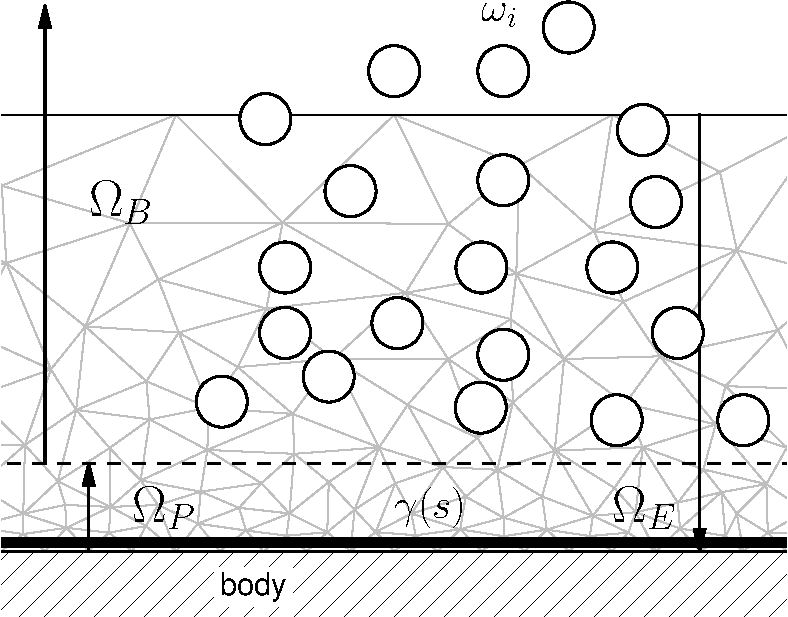
\includegraphics[width=0.45\linewidth]{./figures/hybrid/interpolation/hybrid_domains-crop.pdf}
	\caption{Schematic of the domain decomposition. The two subdomain are the Lagrangian domain $\Omega_L: \Omega_p \cup \Omega_b$ and the Eulerian domain $\Omega_E$ where $\Omega_E \subset \Omega_L$.}
	\label{fig:hybrid_domains}
	\end{figure}

The Lagrangian domain $\Omega_L$ is further divided into two subdomain: the vortex blob domain $\Omega_b$ where the vortex blobs $\mathbf{x}_i \in \Omega_B$ resolve the vorticity $\omega$; and the vortex panel domain $\Omega_p$ consisting of the wall-bounded vorticity resolved by the vortex panel at the surface $\mathbf{s} \in \partial \Omega_{body}$. This division of the Lagrangian domain $\Omega_L$ to $\Omega_b$ and $\Omega_p$ such that $\Omega_L = \Omega_p \cup \Omega_b$ is elaborated in section \ref{sec:boundaryConditions}. The vortex panel was required to efficiently represent the singular vorticity distribution of the wall-bounded vortex sheet and further was necessary to enforce the wall boundary condition for the Lagrangian solver.

Therefore, the decomposition of the fluid domain is as follows:

	\begin{equation}
	\textit{fluid}:\quad\begin{cases}
	\Omega_E &\qquad \text{\{\textit{Eulerian domain}\}}, \\
	\Omega_L = \Omega_p \cup \Omega_b &\qquad \text{\{\textit{Lagrangian domain}\}},
	  \end{cases}
	\end{equation}

and should satisfy the following requirements:
	\begin{itemize}
	\item Eulerian domain belongs to the near-wall region of the Lagrangian domain, $\Omega_E: \Omega_E \subset \Omega_L$, bounded by the wall $\partial \Omega_{body}$ and the exterior Eulerian boundary $\partial \Omega_E$ such that $\Omega_E: \Omega_E \in \left[\partial \Omega_{body}, \partial \Omega_E\right]$.
	\item Vortex panel domain $\Omega_p$ belongs to the near-wall region of the Eulerian domain, $\Omega_p: \Omega_p \subset \Omega_E$, bounded by the wall $\partial \Omega_{body}$ and the boundary $\partial \Omega_p$ such that $\Omega_p: \Omega_p \in \left[\partial \Omega_{body}, \partial \Omega_p\right]$.
	\item Vortex blob domain $\Omega_b$ resolves the off-wall region of the Lagrangian domain $\Omega_b = \Omega_L \backslash \Omega_p$, overlaps with the Eulerian domain $\Omega_b \cap \Omega_E \neq \varnothing$. The vortex vortex blob domains starts from panel exterior boundary $\partial \Omega_p$ and continuous to full fluid domain, $\Omega_b: \Omega_b \in \left[\partial\Omega_p,\infty\right)$.
	\end{itemize}

During the decomposition of the domain, we defined three boundaries, figure \ref{fig:hybrid_config}:
\begin{itemize}
\item $\partial \Omega_{body}$: No-slip wall boundary of the Eulerian domain $\Omega_E$ and the vortex panel domain $\Omega_p$.
\item $\partial \Omega_{p}$: External boundary of the vortex panel domain $\Omega_p$. 
\item $\partial \Omega_E$: External boundary of the Eulerian domain $\partial \Omega_{E}$ where the Dirichlet velocity boundary condition will be prescribed.
\end{itemize}	

%	\begin{figure}[t]
%	\centering
%	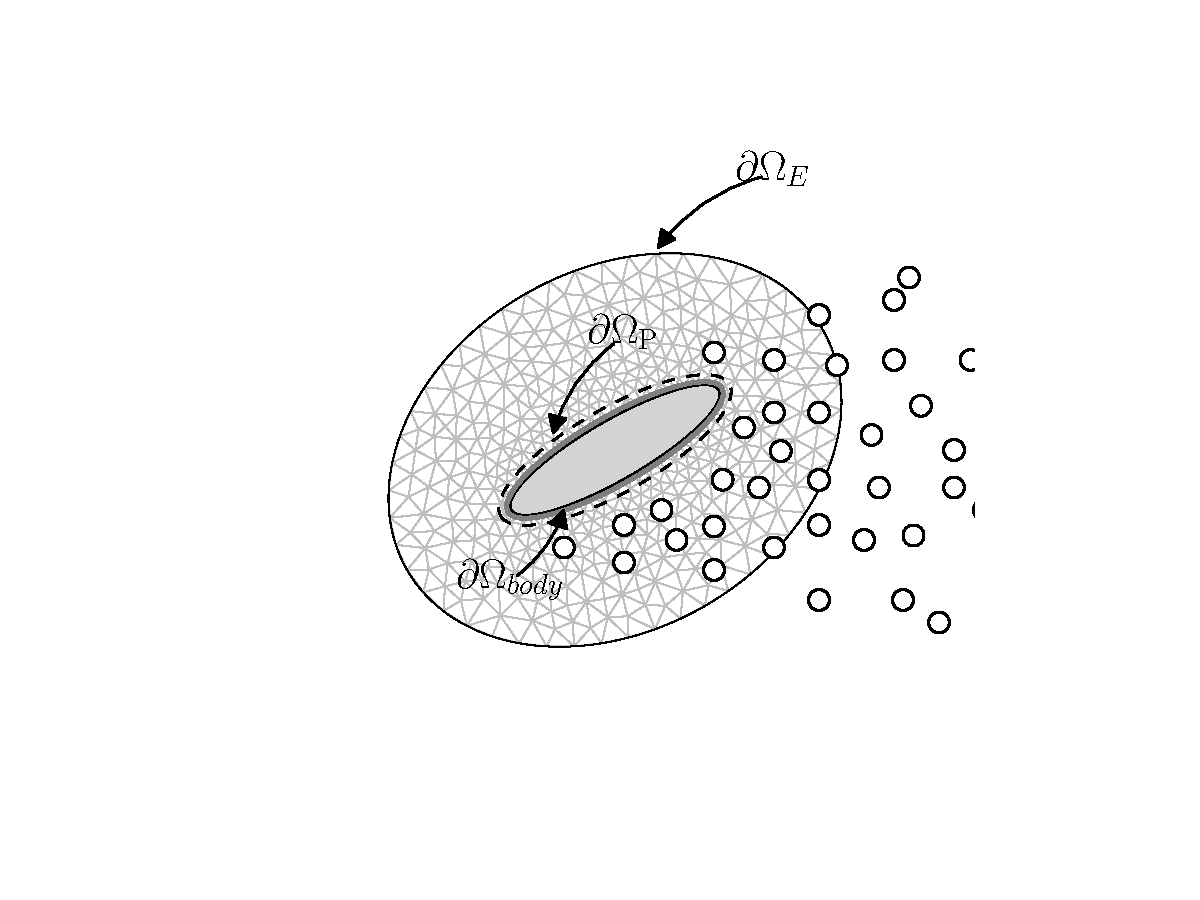
\includegraphics[trim=3.9cm 1.6cm 3.3cm 1.6cm, clip,  width=0.6\linewidth]{./figures/hybrid/interpolation/ellipse/hybrid.pdf}
%	\caption{Boundaries of the decomposed domains. No-slip boundary $\partial \Omega_{body}$, exterior vortex panel boundary $\partial \Omega_p$, exterior Eulerian boundary $\partial \Omega_E$.}
%	\label{fig:hybrid_config}
%	\end{figure}
	
	\begin{figure}[t]
	\centering
	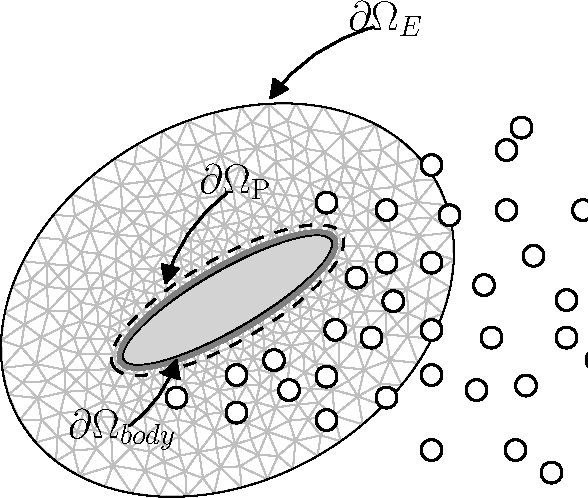
\includegraphics[width=0.5\linewidth]{./figures/hybrid/interpolation/ellipse/hybrid-crop.pdf}
	\caption{Boundaries of the decomposed domains. No-slip boundary $\partial \Omega_{body}$, exterior vortex panel boundary $\partial \Omega_p$, exterior Eulerian boundary $\partial \Omega_E$.}
	\label{fig:hybrid_config}
	\end{figure}		

The solutions in the overlap region $\Omega_E \cap \Omega_L$ will be used to couple the Eulerian and the Lagrangian solver, based on the procedures of Stock \cite{Stock2010a} and the Daeninck \cite{Daeninck2006}.

\subsection{Local to Global Transformation}

The geometries in the simulation are defined in their respective local coordinate system $[x,y]'$. Figure \ref{fig:localPosition} shows an elliptical geometry defined in its local coordinate system about its origin $[{x_o},{y_o}]'$. The origin point is defined such that it is the center of rotation and any rotation will be prescribed about the origin point.

	\begin{figure}[h]
     \centering
     \begin{subfigure}[t]{0.45\textwidth}
             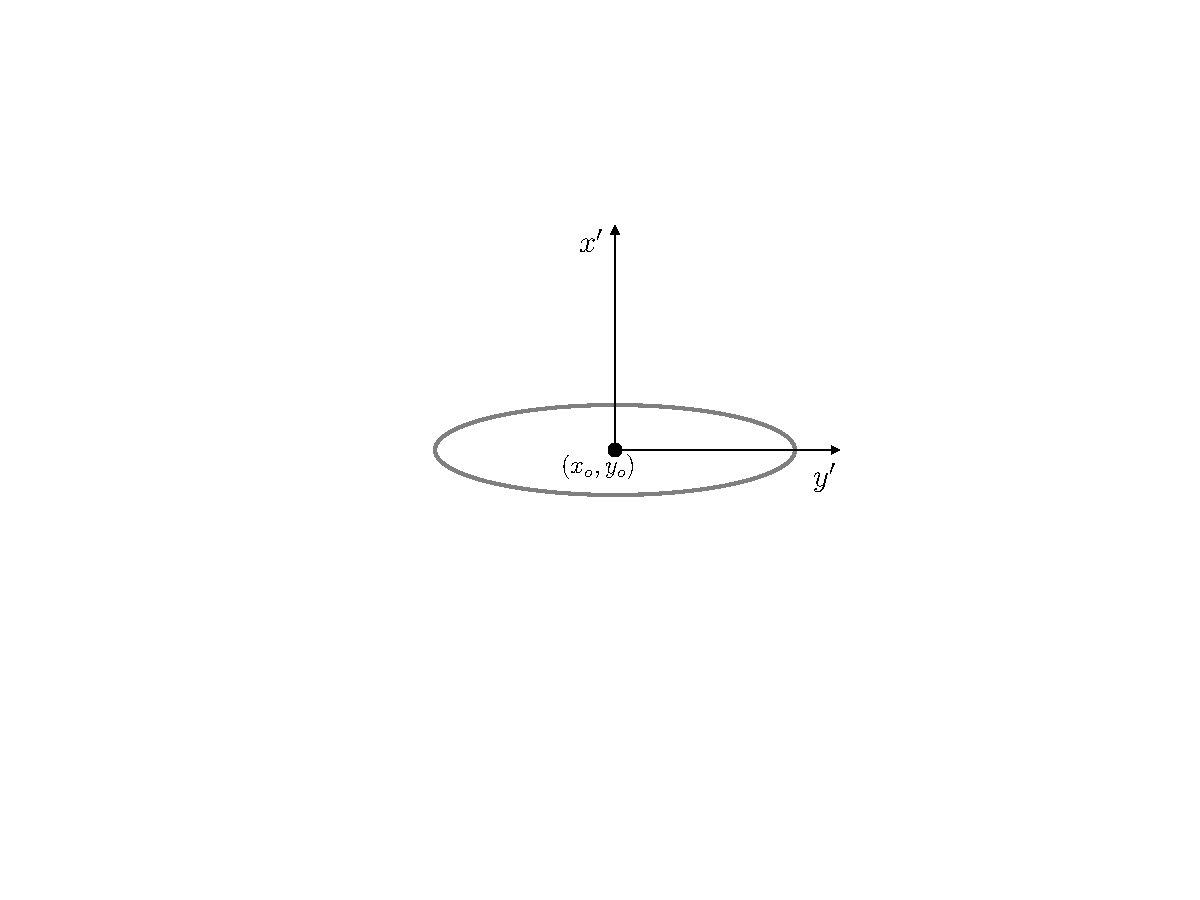
\includegraphics[trim=4.5cm 2.cm 3.5cm 1.5cm, clip, width=\linewidth]{./figures/hybrid/interpolation/ellipse/localOrientation.pdf}
             \caption{Local coordinate system $[x,y]'$}
             \label{fig:localPosition}
     \end{subfigure}%
     ~ %add desired spacing between images, e. g. ~, \quad, \qquad etc.
       %(or a blank line to force the subfigure onto a new line)
     \begin{subfigure}[t]{0.45\textwidth}
             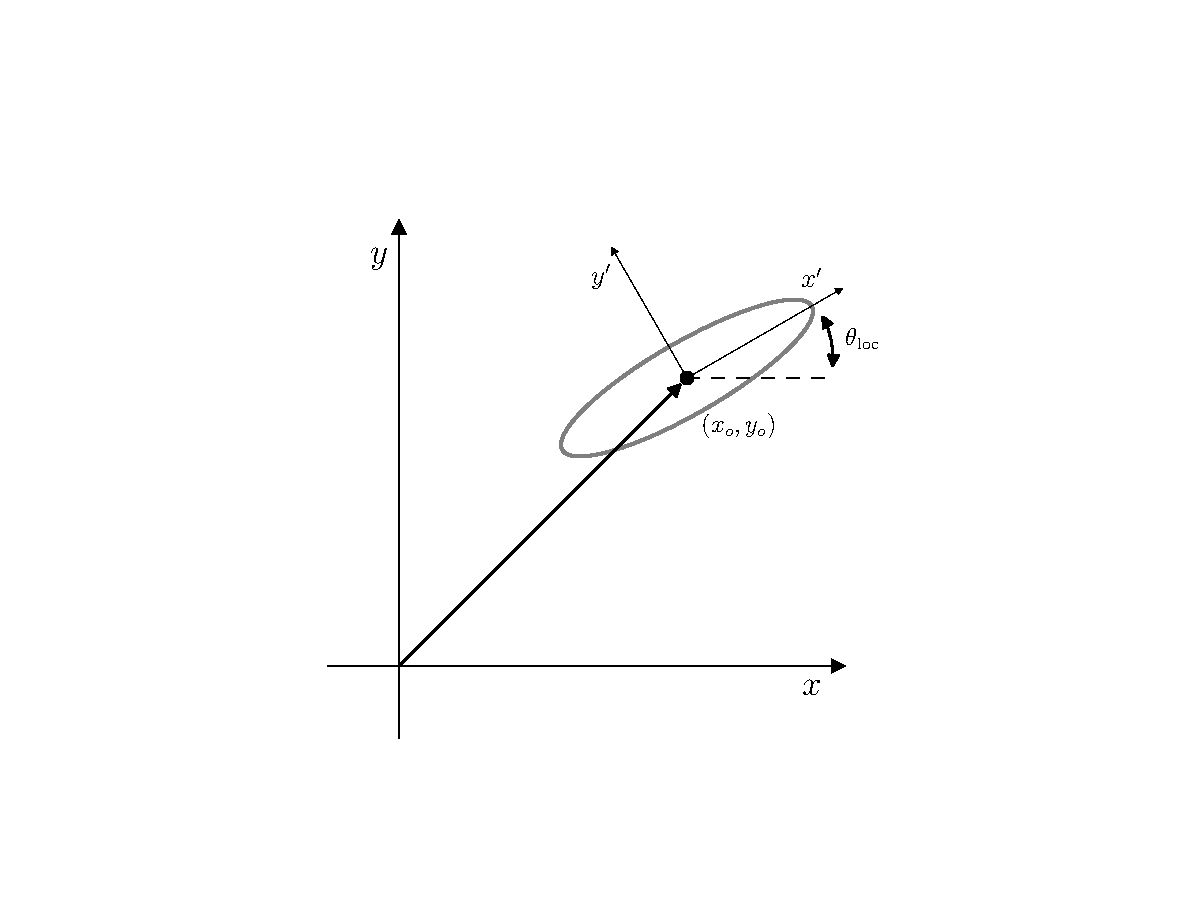
\includegraphics[trim=4.5cm 2.cm 3.5cm 1.5cm, clip, width=\linewidth]{./figures/hybrid/interpolation/ellipse/globalOrientation.pdf}
             \caption{Global coordinate system $[x,y]$}
             \label{fig:globalPosition}
     \end{subfigure}

     \caption{Elliptical geometry in \textbf{(a)} the local coordinate system and \textbf{(b)} the global coordinate system. The geometry is positioned using the displacement vector $[x_o,y_o]$ and rotated by $\theta_0$ about the local origin point.}
     \label{fig:positionOfBody}
	\end{figure}
	
The body is then transformed to the global coordinate system $[x,y]$ by the displacement vector $[x_o,y_o]$ and a local rotation by $\theta_{\mathrm{loc}}$ about the local origin $[x_o,y_o]$. 

The Eulerian solver defines the body mesh in the local coordinate system is then transformed to global position using these parameters. Similarly, the panel geometry for the Lagrangian solver is defined in the same fashion. For a moving problems, the displacement vector and the local rotation angle can be updated to prescribe the motion.


\section{Correction of Lagrangian domain}
\label{sec:correction}
The first step of the hybrid coupling scheme is to transfer the highly resolved Eulerian solution from the Eulerian solver to the Lagrangian solver. The vorticity in the domain $\Omega_E$ is transfered from the grid of the Eulerian solver onto the vortex blobs.
				
\subsection{Approach from literature}		

This is the approach used by Stock \cite{Stock2010a} and is based on the assumption that the Eulerian solution is correct from the body up to `somewhat inside of the outer Eulerian domain", and the Lagrangian solution is correct outside the outer Eulerian boundary. Figure \ref{fig:daeninck_CylinderVorticity} shows Daeninck's \cite{Daeninck2006} result of hybrid coupling. It shows the vorticity field behind a cylinder and at the outer boundary $\partial \Omega_E$ one can observe a slight mismatch in the vorticity, and some artificial vorticity. Daeninck has observed this and stated that this is due to the slight difference in the solution of the two solvers.

	\begin{figure}[h]
	\centering
	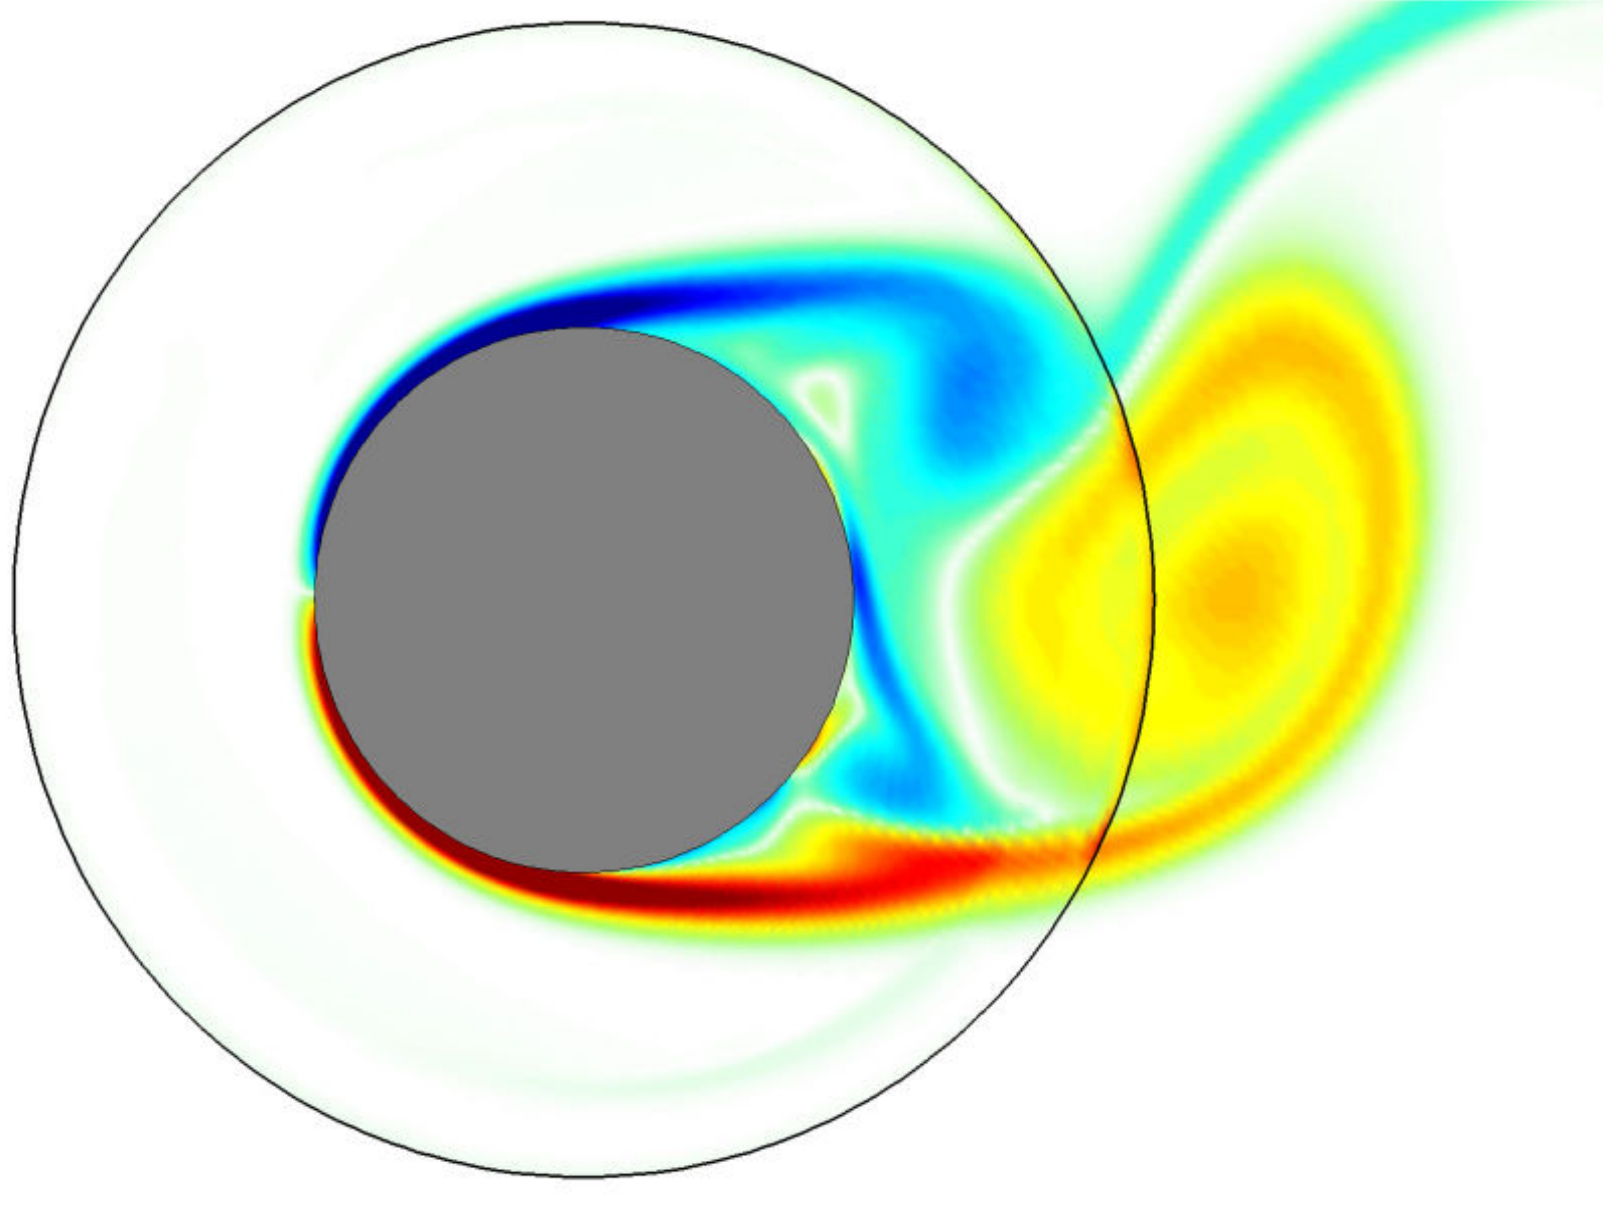
\includegraphics[width=0.5\linewidth]{./figures/hybrid/daeninck_CylinderVorticity.png}
	\caption{Result of hybrid coupling by Daeninck \cite{Daeninck2006}. The figure shows artificial vorticity at the boundary of the Eulerian domain.}
	\label{fig:daeninck_CylinderVorticity}
	\end{figure}

Stock solution to this problem was to interpolate only part of the Eulerian domain of the Eulerian solver onto the Lagrangian solver ignoring the regions of incorrect vorticity field. This introduces the definition of the interpolation region $\Omega_{int}$, as shown in figure \ref{fig:interpRegion}. In addition to the outer boundary region, Stock also proposed to ignore the boundary layer region during interpolation to the vortex blobs. His reasoning for ignoring this region during the correction process was that because the boundary layer has very strong vorticity gradient, they cannot be efficiently represented using the Gaussian vortex kernels. To resolve this singular vorticity distribution, we have to use boundary elements such as the vortex panel kernels, which can efficiently represent such distribution. Therefore, the interpolation region $\Omega_{int}$, figure \ref{fig:interpolationRegionDefinitions}, has the following properties:

	\begin{figure}[!b]
     \centering
     \begin{subfigure}[t]{0.35\textwidth}
             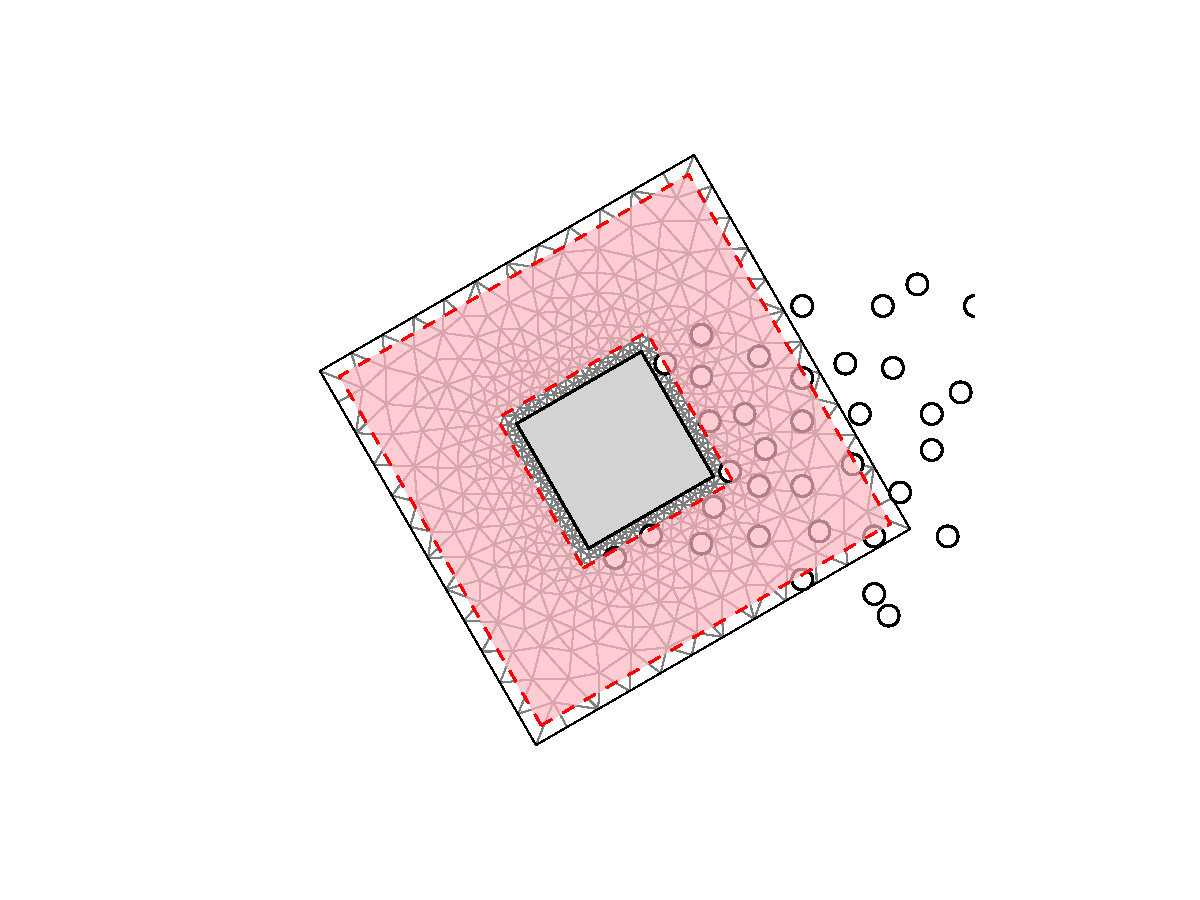
\includegraphics[trim=4.37cm 1.58cm 3.86cm 1.58cm, clip, width=\linewidth]{./figures/hybrid/interpolation/interpRegion.pdf}
             \caption{Boundaries of $\partial \Omega_{int}$}
             \label{fig:interpRegion}
     \end{subfigure}%
     ~ %add desired spacing between images, e. g. ~, \quad, \qquad etc.
       %(or a blank line to force the subfigure onto a new line)
     \begin{subfigure}[t]{0.6\textwidth}
             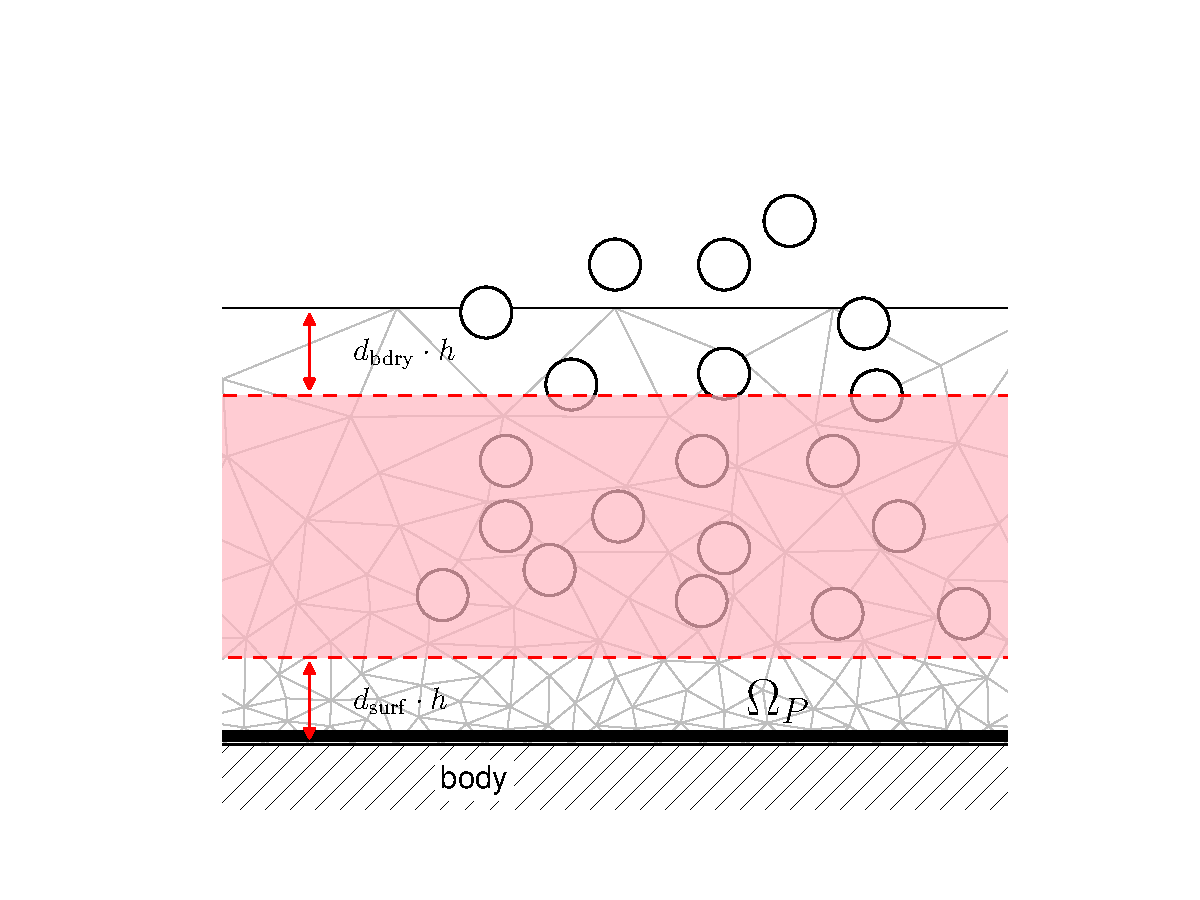
\includegraphics[width=\linewidth]{./figures/hybrid/interpolation/hybrid_domains_withInterpReg.pdf}
             \caption{Offset of the boundaries}
             \label{fig:hybrid_domains_withInterpReg}
     \end{subfigure}

     \caption{Definition of the interpolation region $\partial \Omega_{int}$ with the boundaries: $\partial \Omega_p$ and $\partial \Omega_{int}$.}
     \label{fig:interpolationRegionDefinitions}
	\end{figure}	

	\begin{itemize}
	\item The region is within the overlap region $\Omega_E \cap \Omega_b$ such that $\Omega_{int}: \Omega_{int} \subset \Omega_E \cap \Omega_b$.
	\item The region is starts from the outer vortex panel boundary $\partial \Omega_p$. All the vorticity of the vortex panel boundary is represented using the vortex panels. The interpolation region ends at $\partial \Omega_{int}$, slight distance away from the outer Eulerian boundary $\partial \Omega_E$ ignoring the region of incorrect vorticity, as shown in figure \ref{fig:daeninck_CylinderVorticity}.
	\item The offset of the interpolation region boundaries are in the order of the nominal vortex blobs spacing $h$. The boundary $\partial \Omega_{p}$ is offset by $d_{surf}\cdot h$ from the surface $\partial \Omega_{body}$, where Stock used $d_{surf}=3$. The boundary $\partial \Omega_{int}$ is offset by $d_{bdry}\cdot h$ from the outer Eulerian boundary $\partial \Omega_{E}$, where Stock used $d_{bdry}=2$. 
	\item For an $M'_4$ interpolation kernel and for high Re flows, Stock \cite{Stock2010a}, stated that $d_{surf}=3$ and $d_{bdry}=2$ will ensure proper interpolation of the solutions.
	\end{itemize}

The summary of the interpolation algorithm used by Stock \cite{Stock2010a} based on the works of Daeninck \cite{Daeninck2006} and Guermond and Lu \cite{Guermond2000a} for interpolation the Eulerian solution onto the vortex blobs is as follows:
\begin{enumerate}
\item Interpolate the solution from Eulerian domain onto a temporary structured grid. The temporary structured grid has $\Delta x = \Delta y = h$, the nominal particle spacing and covers the entire Eulerian domain. %Ignore very strong vorticity at the boundary layer, $\mathbf{x} \in \Omega_P$.
\item Identify the particles inside the interpolation region $\Omega_{int}$. Fill gaps in the region with zero-strength particles, so that we can interpolate the Eulerian solution onto them. 
\item Reset the strengths of the particles $\mathbf{x}_i$ inside the interpolation region $\Omega_{int}$, figure \ref{fig:interpRegion}, using the local particle volume and the vorticity interpolated from the grid (i.e $\alpha_i = \omega_i\cdot{h^2}$).
\end{enumerate}

However, during our research we have determined that this approach suffers from some issues and mainly does not guarantee that the circulation is conserved.

\subsection{Issues with the correction algorithm}
\label{subsec:hy_iwtca}
The two main issues with the above approach is as follows:

\begin{itemize}
\item The vorticity bounded to the solid wall was not interpolated to the vortex blobs. 
\item The particle strength initialization using the cell circulation equation, $\alpha_i = \omega \cdot h^2$, does not ensure the local conservation of circulation. %This is the standard approach used by the vortex particle community however, this method does not ensure accurate interpolation of the vorticity field, as described by Barba \& Rossi \cite{Barba2010a}.
\end{itemize}

\subsubsection{Vorticity at the solid wall}

%Therefore to overcome this issue we propose to prescribe the total circulation of the panels such that the circulation is conserved globally.

%\subsubsection*{Prescribed panel strengths}

The first problem that we are concerned is that the vorticity bounded at the solid wall of the Eulerian solver was not transfered to the Lagrangian solver. Stock \cite{Stock2010a} use a Lagrangian solver with BEM that diffuses the vortex sheet to the vortex blobs. However, we implemented the approach of Daeninck \cite{Daeninck2006}, that requires the Eulerian solver to introduced the vorticity generated at the wall to the Lagrangian solver.

To ensure that all the vorticity in fluid is represented, we will use the vortex panels to represents the vorticity of the boundary layer region $\Omega_p$. Furthermore, if the body is at motion, the body will contain circulation do the motion,
	\begin{equation}
	\Gamma_{body} = \iint\limits_{body} \nabla \times \mathbf{u}_b \ \mathrm{d} A.
	\end{equation}

To ensure that all the vorticity is transfered from the Eulerian solver to the Lagrangian solver, we propose to modify Stock's algorithm to transfer the circulation of the domain $\Omega_p$ and the circulation in the body $\Gamma_{body}$ to the vortex panels such that we do not violet the conservation of circulation.

\subsubsection{Vorticity Field interpolation error}
\label{subsubsec:vfie}	
The second issue we must tackle is the interpolation error that arises due to the standard approach of initializing the particles using the local particle volume and the local vorticity,
	\begin{equation}
	\alpha_i = \omega_i\cdot{h^2},
	\end{equation}
where $i$ corresponds to the vortex blobs $\mathbf{x}_i \in \Omega_{int}$. We summarized this issue in the section \ref{subsec:vortexBlobInitialization} of the Lagrangian chapter which was extensively investigated by Barba and Rossi \cite{Barba2010a}. To solve the wake domain of the fluid, we used a vortex particle method that discretizes the vorticity field using $N$ quadrature points,
\begin{equation}
\omega \approx \omega^h(\mathbf{x}_j) = \sum_{i=1}^N \alpha_i \delta(\mathbf{x}_j - \mathbf{x_i}).
\end{equation}

To remove the singularity of the kernel $\delta$, we used a smooth Gaussian kernel $\zeta_{\sigma}$. This approach of using vortex blobs is common in the research of vortex particle method and ensures continuous vorticity distribution. However, the downside to this approach is that on top of the discretization error, we now introduce the ``smoothing error" or the ``regularization error" due to the use of gaussian kernel. This is equivalent to blurring the vorticity field, as explained by Barba and Rossi \cite{Barba2010a}, and the cumulative error in the initialization error is given as:
\begin{equation*}
\mathrm{Error} = \mathrm{Smoothing\  Error} + \mathrm{Discretization\ Error}
\end{equation*}

To perform accurate interpolation of the vorticity $\omega$ inside the interpolation domain $\Omega_{int}$ onto the particles $\mathbf{x}_j \in \Omega_{int}$, we must satisfy the following interpolation problem:
	\begin{equation}
	\left. \omega(\mathbf{x})\  \right|_{\mathrm{Eulerian\ Solver}} = 
	\left. \hat{\omega}(\mathbf{x})\  \right|_{\mathrm{Lagrangian\ Solver}},
	\end{equation}
where the $\left. \omega(x) \right|_{\mathrm{Eulerinan\ Solver}}$ is the Eulerian solution from the Eulerian solver, and the smoothed Lagrangian vorticity from the Lagrangian solver is given as,
	\begin{equation}
	\hat{\omega}(\mathbf{x}) = \sum_{i=1}^{N} \alpha_i \zeta_{\sigma}(\mathbf{x} - \mathbf{x}_i).
	\label{eq:mollifiedVorticityDistributionEquation}
	\end{equation}
The discrete vorticity field is represented by the linear combinations of the Gaussian basis function $\zeta_{\sigma}$ with the vortex blob strength $\alpha_i$. Therefore taking that $\alpha_i = \omega(\mathbf{x}_i)\cdot{h^2}$ is mathematically incorrect and does not ensure the interpolated vorticity field matches the original vorticity distribution from the Eulerian solver.

We discussed the Beale's iterative method for retaining the original vorticity distribution in section {\color{plotRed}{?????}} \ref{subsubsec:BealesMethod}, however this approach cannot be employed for decomposed domains. The Beale's method uses equation \ref{eq:mollifiedVorticityDistributionEquation} to construct a linear system of equation to directly solve for the particle strengths $\alpha_i$:
\begin{equation}
\mathbf{A}_{ij}\alpha_i = \omega_i,
\end{equation}
where the coefficient matrix $\mathbf{A}$ is given as,
\begin{equation}
\mathbf{A}_{ij} = \zeta_{\sigma}(\mathbf{x}_j-\mathbf{x}_i).
\label{eq:initialization}
\end{equation}

However inverting the matrix $\mathbf{A}$ is still an open question, as stated by Koumoutsakos and Cottet \cite{Cottet2000a}, and was the primary investigation of Barba and Rossi \cite{Barba2010a}. The problem is that the matrix $\mathbf{A}$ is full and badly condition for direct inversion. For a global field interpolation (i.e for unbounded domain), one could use the Beale's iterative method which uses a \printAcron{successive over-relaxation}{SOR} for solving the equation \ref{eq:initialization}. This method relies on iterative correction of all the particles $\mathbf{x}_i \in \Omega_L$, in the full Lagrangian domain. However, in our case of initializing the strengths of the particles $\mathbf{x}_i$ in the sub-domain $\Omega_{int}$ of the Lagrangian domain $\Omega_L$, it would require us to modify the strength of only the particles $\mathbf{x}_i$ in $\Omega_b$. In such case, the Beale's iterative method is not valid and cannot be used. Therefore, the Beale's method cannot be used to solve the problem of the smoothing error.

In future, the key to solving this smoothing error might be in the research works of Barba and Rossi \cite{Barba2010a}, where they try to reverse the blurring of the vorticity field by reversing the ``diffusion" caused by the smoothing kernel. However, currently for our investigation the best possible way of ensure minimal interpolation error from Eulerian domain onto vortex blobs is to perform the following steps:
\begin{itemize}
\item Minimize the smoothing and discretization error by maximizing the particle resolution, achieved by setting $Ov=1$ and reducing $\sigma$ such that the relative error $\epsilon \leqslant 5\%$. The convergence of the overlap $Ov$ and the core spreading $\sigma$ was investigated in section \ref{subsubsec:convergenceInterpolation}.
\item A vital requirement for vortex particle method is the conservation of circulation. Therefore, to ensure that the Hybrid method is valid, we ensure that the interpolation of the vorticity from the Eulerian solver to the Lagrangian solver satisfies the conservation of circulation.
\end{itemize}

Thus, we will modified the approach of Stock \cite{Stock2010a} to ensure that all the vorticity in transfered from the Eulerian solver to the Lagrangian solver and that we satisfy the conservation of circulation.

\subsection{Modified correction strategy}
\label{subsec:mcs}
The modified version of the correction can be divided into five steps
\begin{enumerate}
\item \textbf{Probe vorticity}: Interpolate the vorticity from the unstructured Eulerian mesh onto a uniform structured grid.
\item \textbf{Remove particles}: Remove particles that are inside the interpolation domain $\Omega_{int}$.
\item \textbf{Generate particles}: Generate zero-strength particle inside the interpolation domain $\Omega_{int}$.
\item \textbf{Assign strengths}: Use the standard particle initialization approach, $\alpha_i = \omega_i \cdot h^2$ to assign the particles $\mathbf{x}_i$.
\item \textbf{Conserve circulation}: Determine the mismatch in the total circulation of the Lagrangian field as determine the strength of the panels such that circulation is conserved.
\end{enumerate}

\subsubsection*{Probe vorticity}

The first sub-step of the correction step is to interpolate the vorticity from the unstructured Eulerian grid onto a uniform structured grid. The purpose of the structured grid is to perform fast and efficient interpolation of vorticity from the Eulerian domain onto the vortex blobs. 

	\begin{figure}[h]
	\centering
	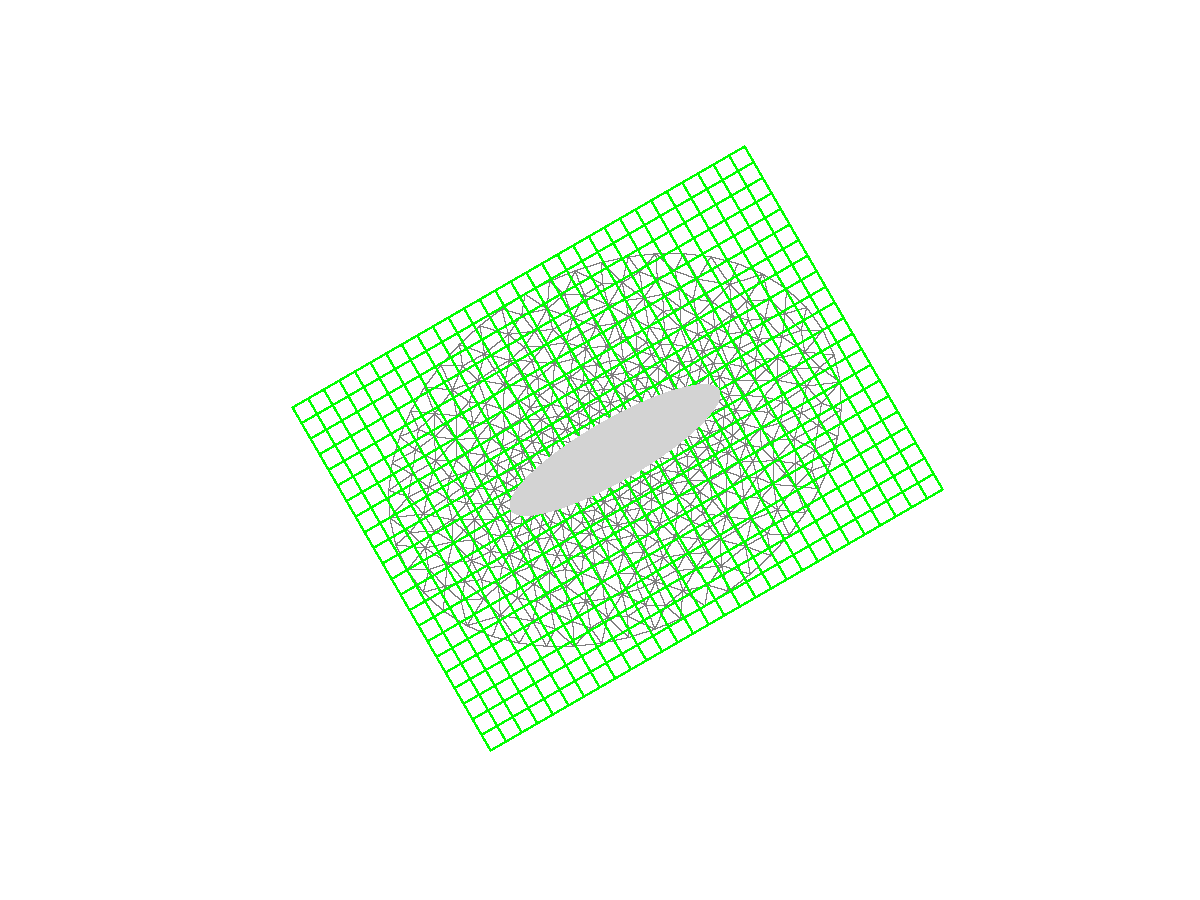
\includegraphics[trim=4.37cm 1.58cm 3.86cm 1.58cm, clip, width=0.5\linewidth]{./figures/hybrid/interpolation/ellipse/interpolation_FE2andStructuredGrid.pdf}
	\caption{Structured interpolation grid $\mathbf{x}_{str}$ (pink) covering the entire Eulerian mesh (gray).}
	\label{fig:interpolation_FE2andStructuredGrid}
	\end{figure}	
	
The structured grid $\mathbf{x}_{str}$ is defined in the local coordinates system of the geometry $[x,y]'$ where the grid covers the entire Eulerian domain $\Omega_E$. Figure \ref{fig:interpolation_FE2andStructuredGrid} shows the structured grid bounded to the Eulerian domain in the global coordinate system. The vorticity function $\omega$ of the function space $X$ of the Eulerian solver is interpolated from the unstructured mesh $\mathbf{x}_{\mathrm{unstr}}$ onto the structured uniform grid $\mathbf{x}_{\mathrm{str}}$,
	\begin{eqnarray}
	\hat{\omega}_i = \sum_k \omega_k W_{ki}
	\end{eqnarray}
using the interpolation weight $W$, where $\hat{\omega}$ is the interpolated vorticity. Figure \ref{fig:interpolation_FE2StructuredGrid_withData} shows a depiction of the transfer of the vorticity from the unstructured grid to the structured grid. As the structured grid $\mathbf{x}_{str}$ that does not move w.r.t to the unstructured mesh $\mathbf{x}_{unstr}$, the interpolation weight $W$ only needs to be calculated once, ensuring fast interpolation. We used the \texttt{Probe} function, a C++ implementation developed by Mortensen \cite{fenicstools}, to the probe the vorticity function space $X$ for the structured vorticity $\hat{\omega}$ at the nodes of the structured grid $\mathbf{x}_{str}$.

	\begin{figure}[h]
	\centering
	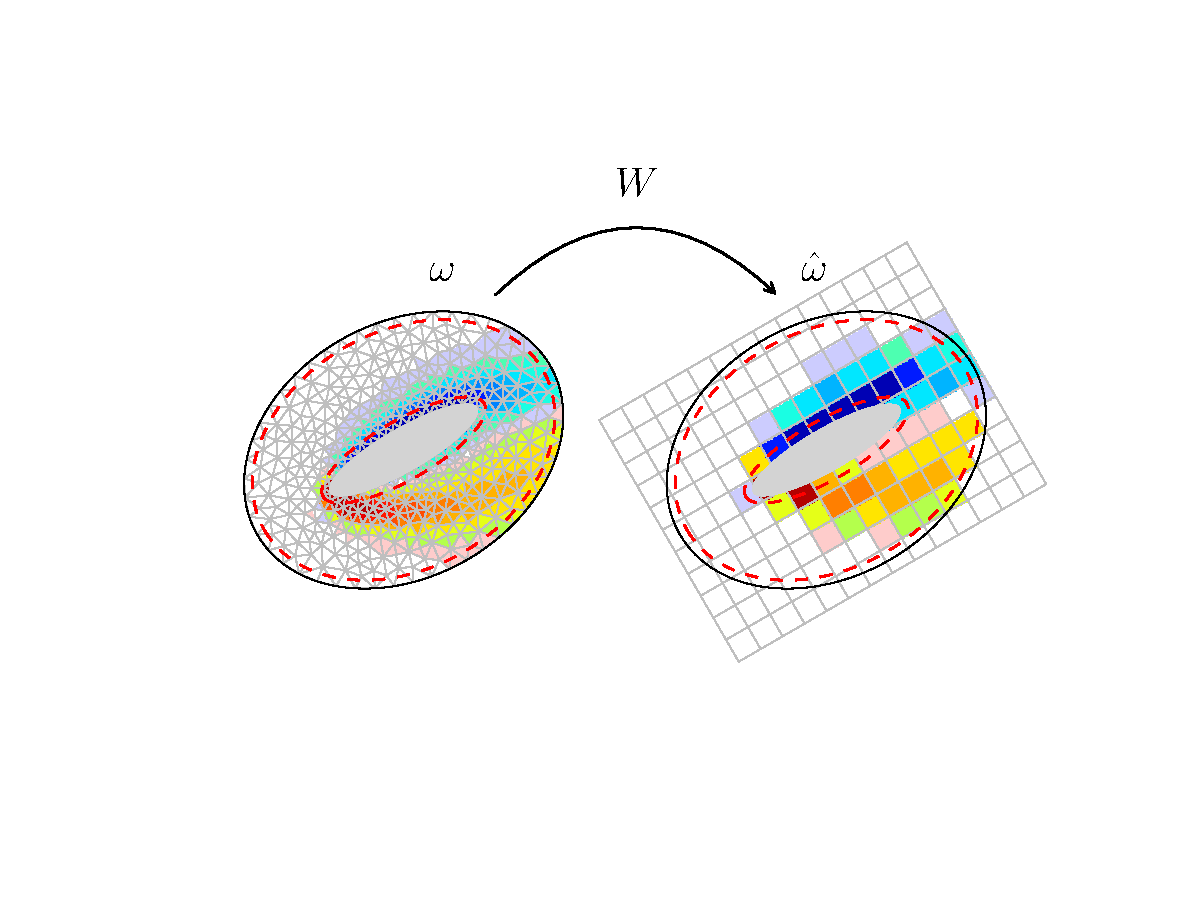
\includegraphics[trim=4.cm 4cm 2cm 2.5cm, clip, width=0.7\linewidth]{./figures/hybrid/interpolation/ellipse/interpolation_FE2StructuredGrid_withData.pdf}
	\caption{Interpolated vorticity $\hat{\omega}$ on the structured grid $\mathbf{x}_{str}$ from interpolating $\omega$ of the unstructured grid $\mathbf{x}_{unstr}$ with the interpolation weights $W$.}
	\label{fig:interpolation_FE2StructuredGrid_withData}
	\end{figure}

Once we have determine $\hat{\omega}$, we can assign the strengths of the particles using an efficient index search algorithm to find the location of the particle in the structured grid. If we had not used this approach and directly transfered the vorticity from the unstructured mesh $\mathbf{x}_{unstr}$ onto the vortex blobs $\mathbf{x}_i$, at each iteration we would require an expensive search algorithm to determine the position of the blob w.r.t to the nodes of the unstructured grid. This would mean that we would have to construct the interpolation matrix at each iteration, drastically reducing the efficiency of interpolation.

\subsubsection*{Remove particles}

	\begin{figure}[!b]
     \centering
     \begin{subfigure}[t]{0.49\textwidth}
             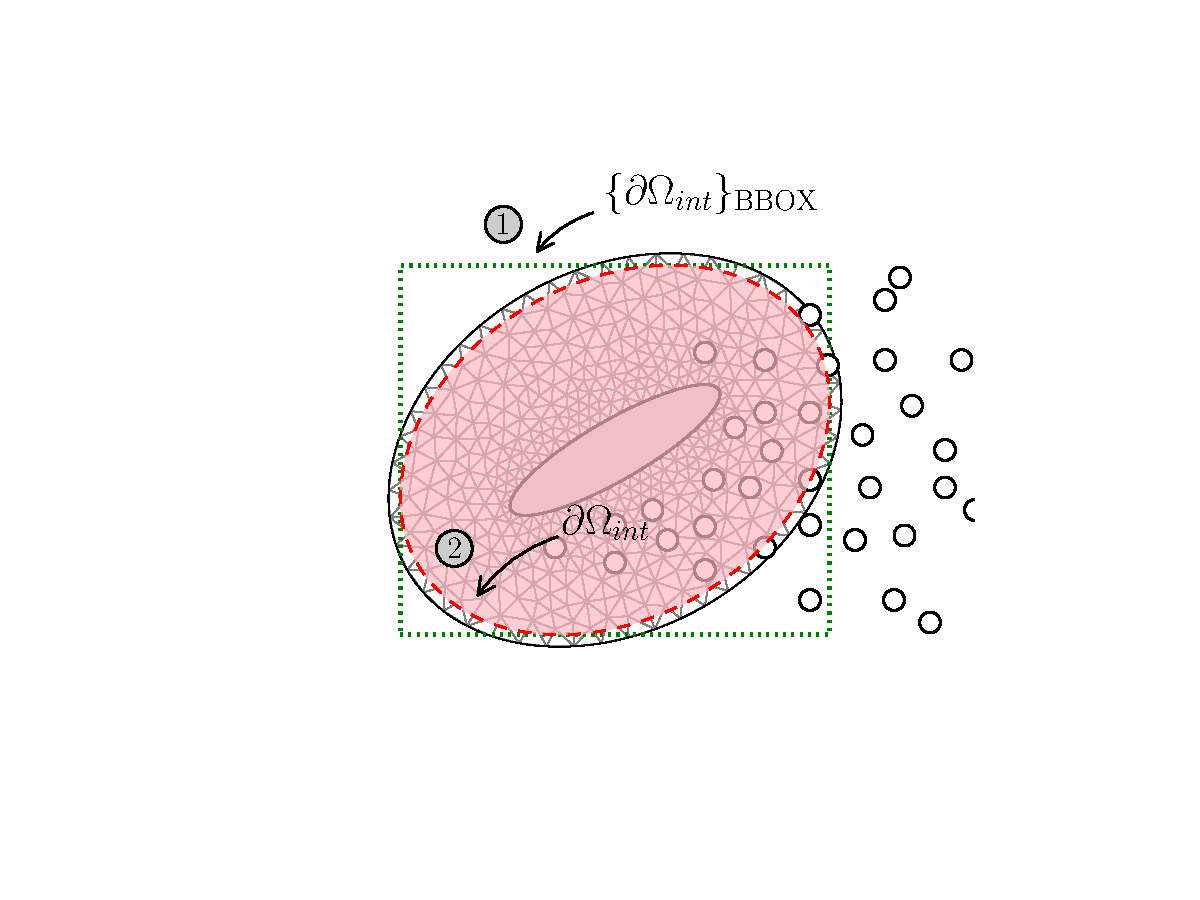
\includegraphics[trim=4.37cm 1.58cm 3.86cm 1.58cm, clip, width=\linewidth]{./figures/hybrid/interpolation/ellipse/interpRegion.pdf}
             \caption{Particles inside the interpolation region}
             \label{fig:region}
     \end{subfigure}%
     ~ %add desired spacing between images, e. g. ~, \quad, \qquad etc.
       %(or a blank line to force the subfigure onto a new line)
     \begin{subfigure}[t]{0.49\textwidth}
             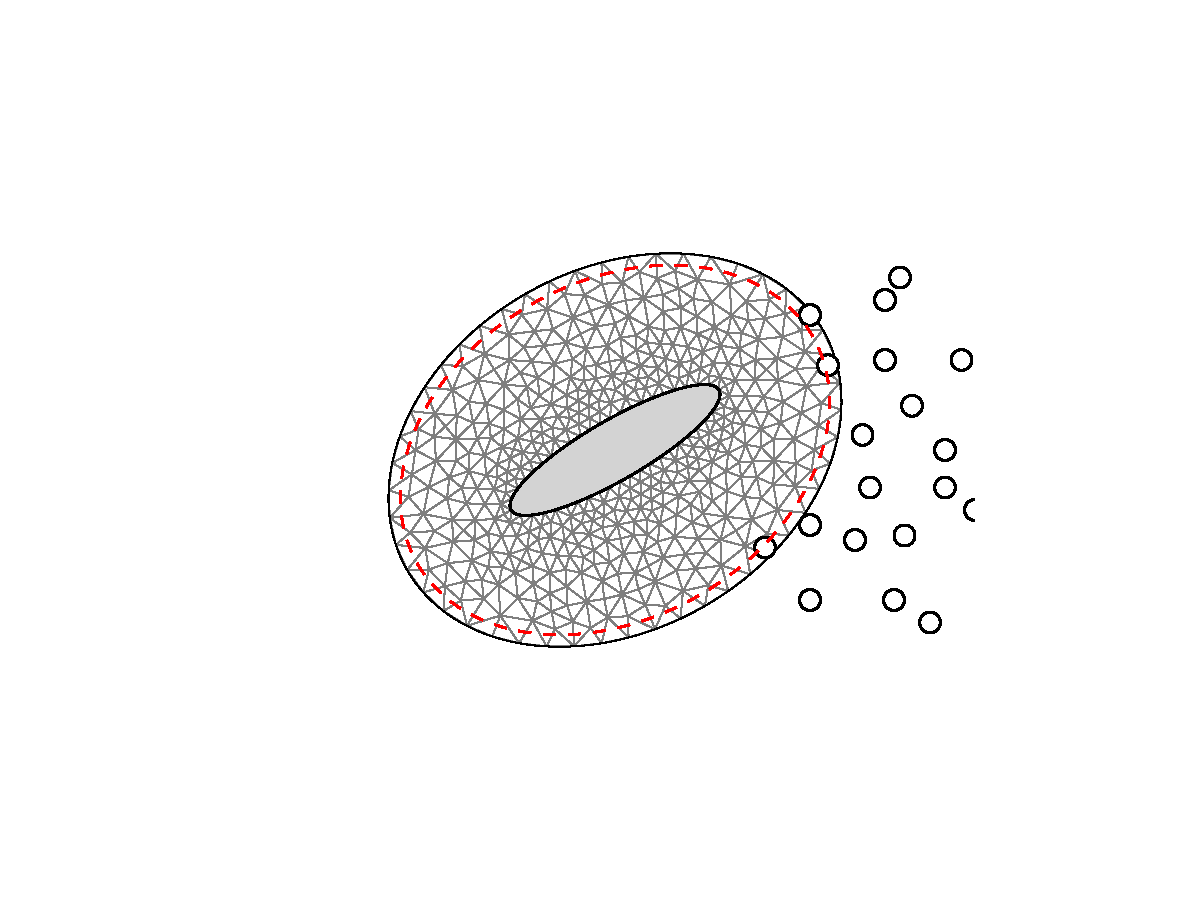
\includegraphics[trim=4.37cm 1.58cm 3.86cm 1.58cm, clip, width=\linewidth]{./figures/hybrid/interpolation/ellipse/particleRemoved.pdf}
             \caption{Total circulation $\Gamma_{removed}$ removed.}
             \label{fig:removed}
     \end{subfigure}

     \caption{The interpolation region $\Omega_{int}$, bounded by the boundary polygons: panel region boundary $\partial \Omega_P$ near the wall, and exterior boundary $\partial \Omega_{int}$ near the outer region.}
     \label{fig:interpRegionEllipse}
	\end{figure}	

The second sub-step of the correction step is remove the particles that are inside the interpolation region $\Omega_{int}$ and the vortex panel domain $\Omega_p$. The purpose of this step is that we want to ultimately correct the Lagrangian solution in these regions with the more refined Eulerian solution of the domain $\Omega_E$. To perform the coupling, we first need to remove the particles in the region of correction $\Omega_{int}$ and $\Omega_p$. Figure \ref{fig:region} shows the vortex blobs $\mathbf{x}_i$ inside the boundary $\partial \Omega_{int}$ that needs to be removed. To see which particles are inside, we need to perform a ``Point inclusion in polygon" test to determine which particles $\mathbf{x}_i$ are within the boundary polygon $\partial \Omega_{int}$. However, this point-in-polygon search is computationally expensive but can be simplified by neglecting the particles outside the minimum bounding box of the polygon. Thus the steps to remove the vortex blobs inside the interpolation region is as follows:
\begin{enumerate}
\item Determine which particles inside the bounding box of the polygon $\partial \Omega_{int}$. 
\item Perform a point-in-polygon test for only the particles $\mathbf{x}_i \in \mathrm{BBOX}\{\partial \Omega_{int}\}$.
\item Remove the particles $\mathbf{x}_i$ from the total set of particles, resulting in a total circulation change of $\Gamma_{removed}$.
\end{enumerate}

To perform the point-in-polygon test, we used the \texttt{pnpoly} function of \texttt{matplotlib}, the python 2D plotting library created by Hunter \cite{Hunter:2007}. The function implemented the ``point inclusion in polygon" test algorithm developed by Franklin \cite{franklin2006pnpoly}. The algorithm is based on the crossings test, which determines whether the point is inside the polygon by determining the number of the times a semi-infinite ray originating from the point intersects with the polygon.

\subsubsection*{Generate particles}

The third sub-step of the correction step is generate zero-strength particles inside interpolation region $\Omega_{int}$, figure \ref{fig:generatedParticles}. These zero-strength particles will later be corrected with the strengths obtained from the structured grid $\mathbf{x}_{str}$.

	\begin{figure}[h]
	\centering
	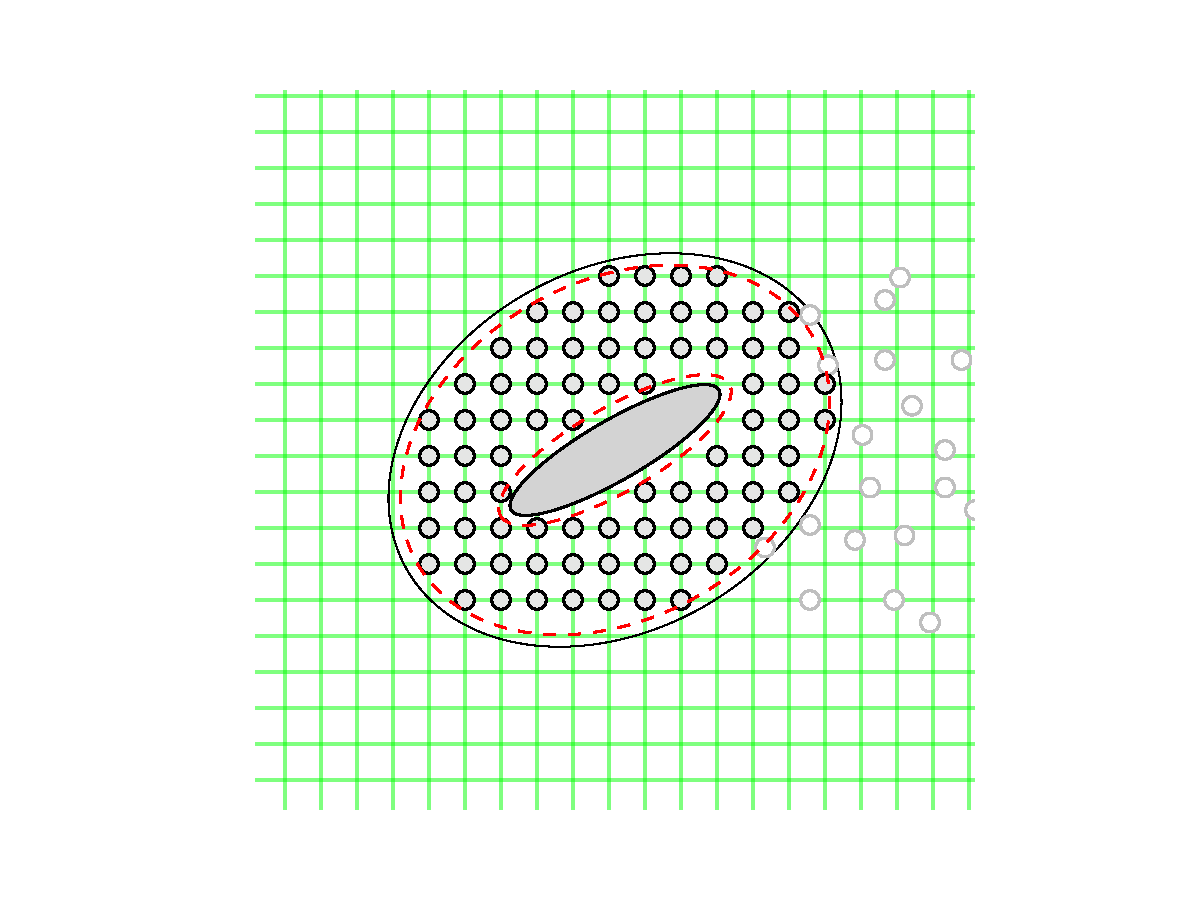
\includegraphics[trim=4.37cm 2.3cm 4.cm 2.cm, clip, width=0.5\linewidth]{./figures/hybrid/interpolation/ellipse/generatedParticles.pdf}
	\caption{Particles inside the interpolation domain $\Omega_{int}$ located at $\mathbf{x}_i$ coinciding the Lagrangian remeshing grid.}
	\label{fig:generatedParticles}
	\end{figure}

The procedures of generating zero-strength particles are as follows:
\begin{enumerate}
\item Generate zero-strength particles $\mathbf{x}_i$ inside the bounding box of the boundary polygon $\partial \Omega_{int}$, $\mathbf{x}_i \in \mathrm{BBOX}\{\partial \Omega_{int}\}$. The position of the particles $\mathbf{x}_i$ coincides with the global Lagrangian remeshing grid (shown in green), such that particles are equally spaced.
\item Perform a point-in-polygon test for the particles $\mathbf{x}_i$, so that we can neglect the particles outside of the interpolation boundary $\partial \Omega_{int}$, the particles inside the body $\Omega_{\mathrm{body}}$, and the particles inside the vortex panel domain $\Omega_p$, leaving us only the particles $\mathbf{x}_i \in \Omega_{int}$.
\end{enumerate}

Figure \ref{fig:generatedParticles} shows the newly generated particles (in black) and the pre-existing set of particles (in gray). Onces we have uniformly distributed particles covering all the regions of the interpolation region $\Omega_{int}$, we can transfer the solution from the Eulerian solver to the Lagrangian solver.

\subsubsection*{Assign strengths}

	\begin{figure}[!b]
	\centering
	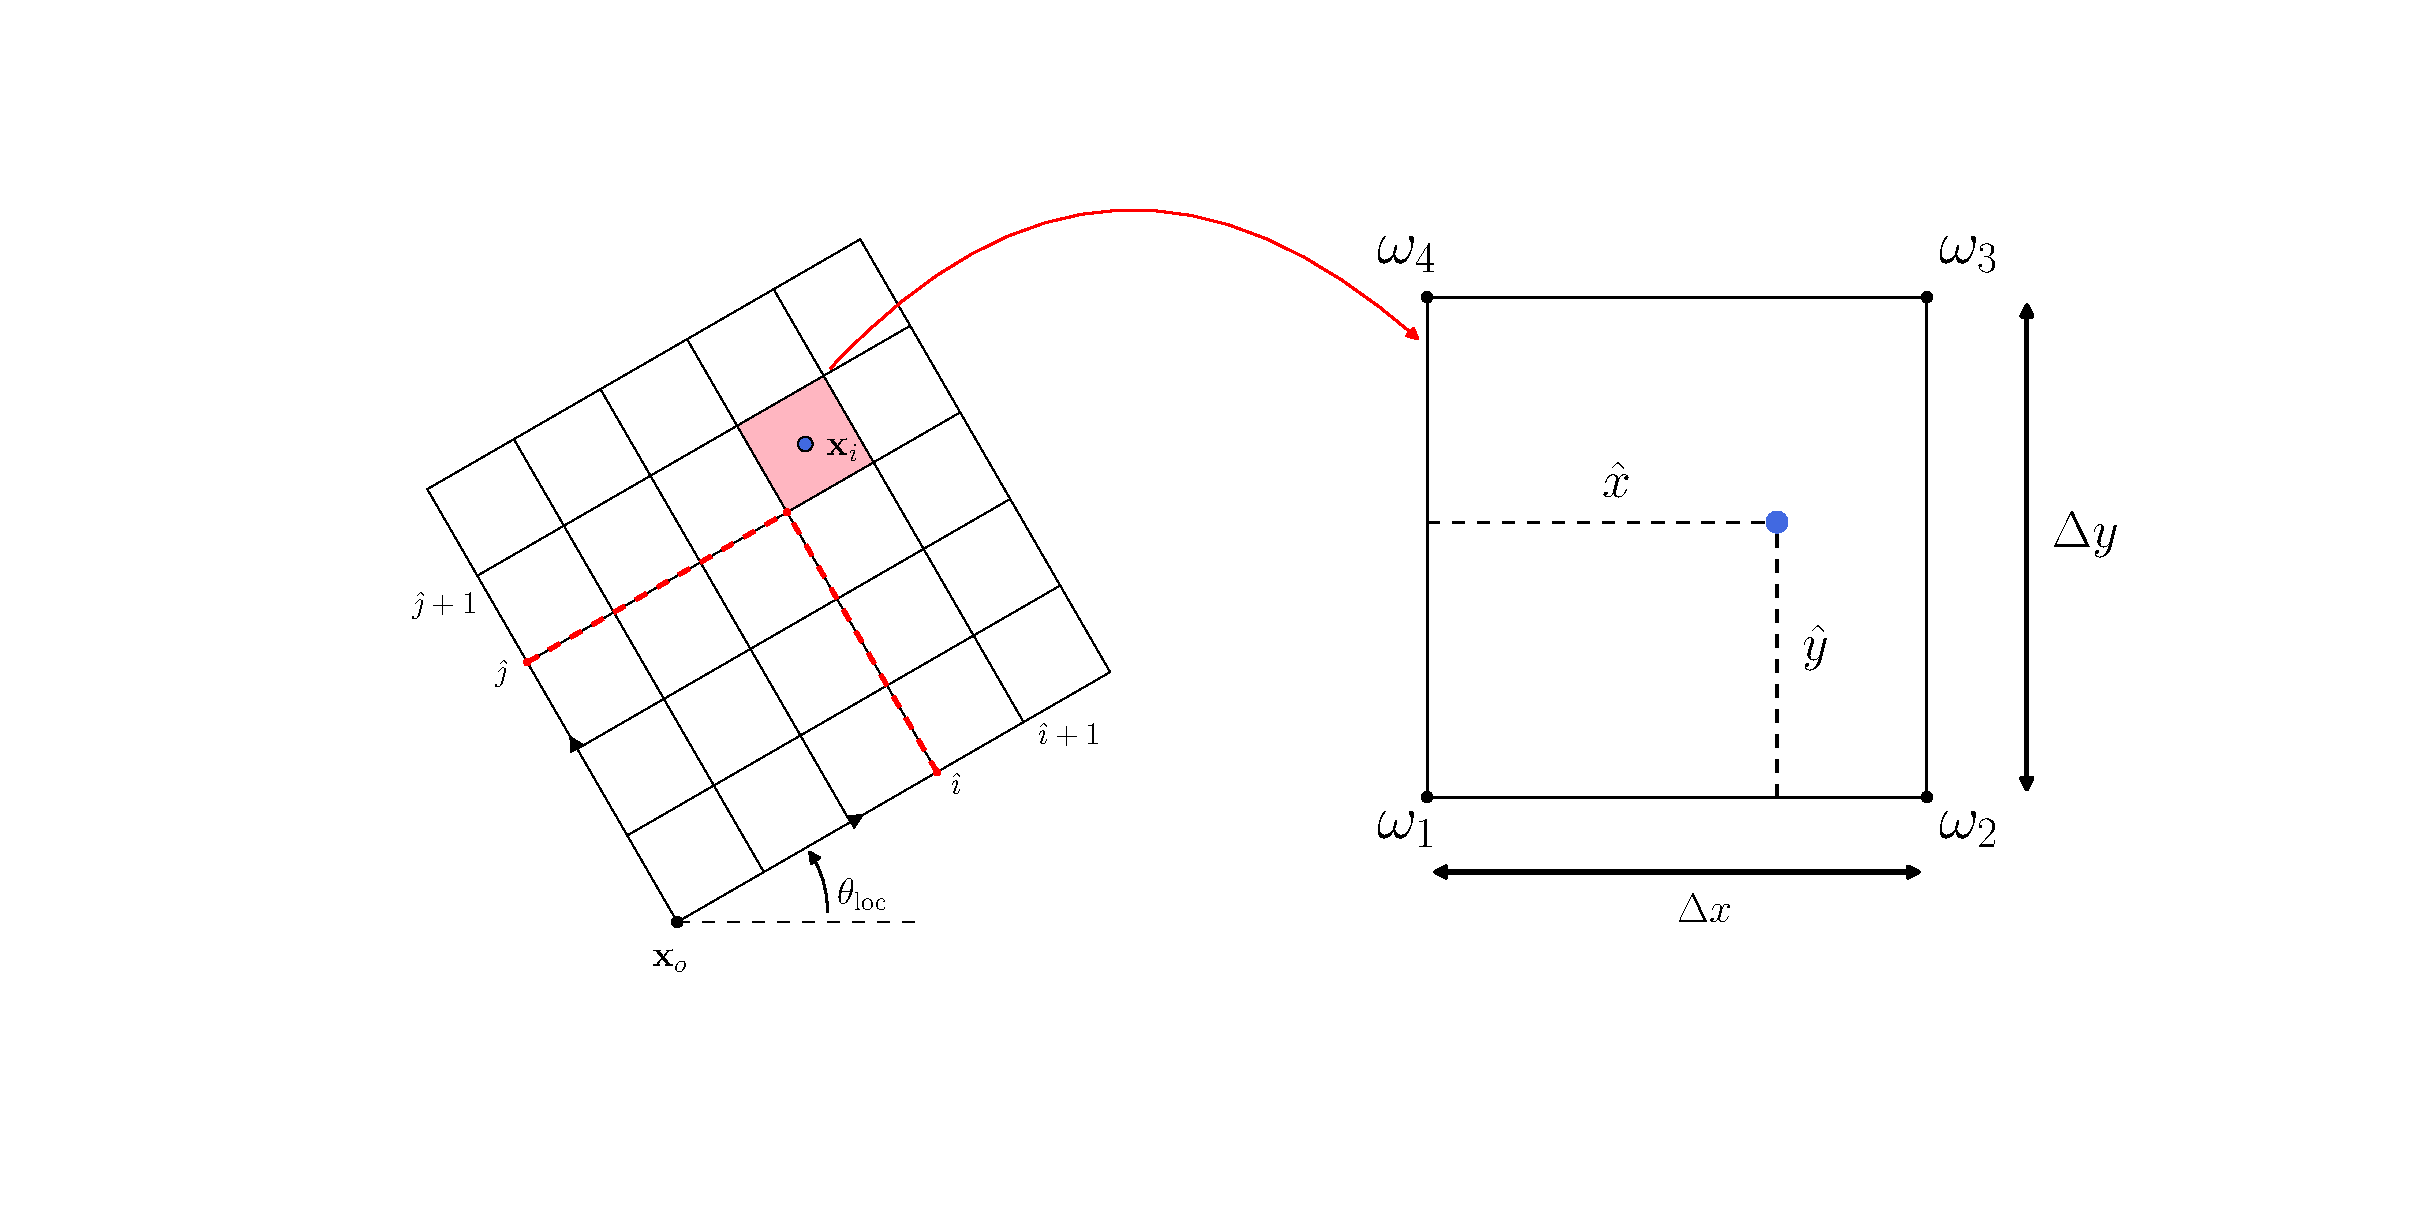
\includegraphics[trim=5.5cm 3.cm 4.5cm 3cm, clip, width=0.99\linewidth]{./figures/hybrid/interpolation/ellipse/interpolationManual.pdf}
	\caption{Interpolating the strengths from the structured grid $\mathbf{x}_{str}$ onto the vortex blobs $\mathbf{x}_i$ using a bilinear interpolation}
	\label{fig:interpolationManual}
	\end{figure}


The fourth sub-step of the correction is to assign the strengths to the newly generated particles in the interpolation domain $\Omega_{int}$. The strengths of the particles $\alpha_i$ is determined using the standard method,
\begin{equation}
\alpha(\mathbf{x}_i) = \hat{\omega}(\mathbf{x}_i) \cdot h^2,
\end{equation}
where the local circulation inside the area $h^2$ is assigned to the particle. We have minimized the $h^2$ interpolation area such that the smoothing error caused the Gaussian kernel is acceptable, see section \ref{subsubsec:convergenceInterpolation}. Therefore, to determine the strength of the particles inside the interpolation region, we simply require the vorticity $\hat{\omega}(\mathbf{x}_i)$ at the local $\mathbf{x}_i$. We have interpolated the vorticity from the unstructured finite element grid nodes onto a structure grid $\mathbf{x}_{str}$. We can transfer the vorticity from the structured grid onto to vortex blobs using an efficient Bilinear interpolation algorithm.



Figure \ref{fig:interpolationManual} shows the schematic representation of the Bilinear interpolation of vorticity. The vortex blob (in blue) is located inside the one of the cells of the structured grid (in pink), bounded by 4 grid nodes:
\begin{eqnarray}
\begin{aligned}
p_1 &= \mathbf{x}_{i,j},\\
p_2 &= \mathbf{x}_{i+1,j},\\
p_3 &= \mathbf{x}_{i+1,j+1},\\
p_4 &= \mathbf{x}_{i,j+1}.
\end{aligned}
\end{eqnarray}

	\begin{figure}[!b]
	\centering
	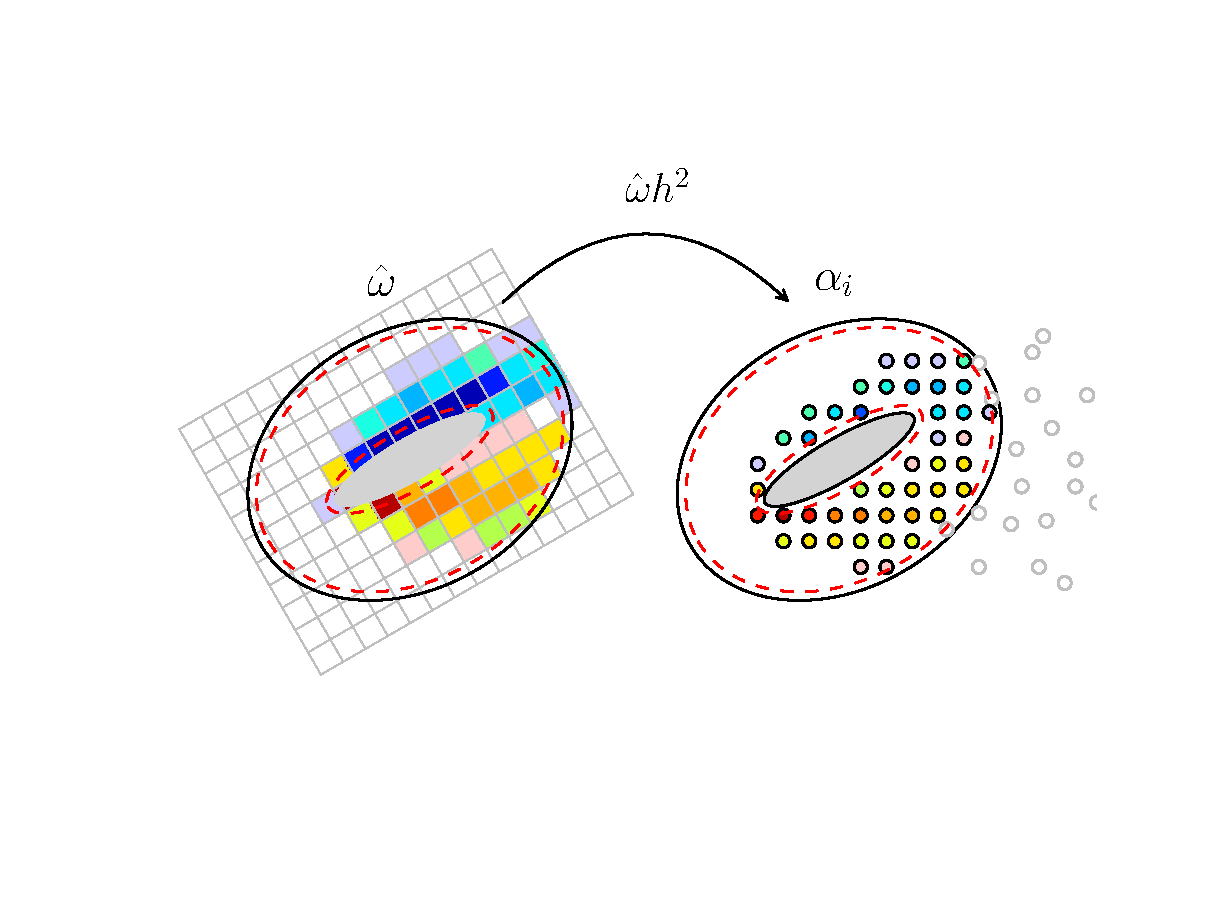
\includegraphics[trim=2.55cm 3.35cm 2.05cm 2.5cm, clip, width=0.9\linewidth]{./figures/hybrid/interpolation/ellipse/interpolation_StructuredGrid2Blobs.pdf}
	\caption{Interpolated strengths $\alpha_i$ from the structured grid $\mathbf{x}_{str}$ using bilinear interpolation.}
	\label{fig:interpolation_StructuredGrid2Blobs}
	\end{figure}	

The four nodes $p_1,...,p_4$ are defined in the anti-clockwise direction. The bilinear interpolation of the vorticity becomes,
	\begin{equation}
	\hat{\omega}(\mathbf{x}_i) = \sum_{k=1}^4 W_k\cdot \omega_k
	\end{equation}
where $\{\omega_k, W_k\} \mapsto p_k$. The interpolation weights $W_k$ are defined as 
	\begin{equation}
	\begin{aligned}
	W_1 &= \frac{(\hat{x} - \Delta x )(\hat{y}-\Delta y)}{\Delta x \Delta y}\\
	W_2 &= \frac{-\hat{x}(\hat{y}-\Delta y)}{\Delta x \Delta y}\\
	W_3 &= \frac{\hat{x} \hat{y}}{\Delta x \Delta y}\\
	W_4 &= \frac{-\hat{y}(\hat{x} - \Delta x )}{\Delta x \Delta y}
	\end{aligned}
	\end{equation}

	
where the cell of the structured grid has dimension $[\Delta x, \Delta y]$, with $\Delta x= \Delta y$. The coordinates of the blobs are normalized such that, the vortex blobs is located at $0\leqslant\hat{x}\leqslant\Delta x$ and $0\leqslant\hat{y}\leqslant\Delta y$. Figure \ref{fig:interpolation_StructuredGrid2Blobs} shows the results of the assigning the strengths of the particles from the structured grid. 
	
\subsubsection*{Conserve circulation}
\label{subsubsec:cc}
The fifth and the final step of correcting the Lagrangian filed is to ensure that the we have to ensure that circulation is conserved. Two main source of errors for the conservation of circulation is the vorticity at the solid wall, and the vorticity field interpolation error.

The vorticity at the solid was not transfered to particles because the Gaussian kernels cannot efficiently represent the singular distribution. However, we cannot simply neglect this distribution and therefore we use the vortex panels to represent these. To ensure that the conservation of circulation is satisfied in the Lagrangian solver, we will prescribe the integral strengths of the panels (i.e the total circulation).

The second error is the vorticity field interpolation error. The correction algorithm so far does satisfy the conservation of circulation, so we will employ Kelvin's circulation theorem to ensure circulation is conserved. If we are dealing with fluid flow with initial total circulation $\Gamma_0 = 0$, then according to Kelvin's circulation theorem, we require that at all times $t$,
\begin{equation}
\Gamma_{panels} + \Gamma_{blobs} = 0.
\end{equation}

Thus, to ensure that the circulation is conserved, we have to solve for the no-slip panels such that the total circulation is zero. However, in a general case (especially when we are dealing with multiple bodies), we have to formulate the equality in a different manner. We have to define two regions of the flow, domain where Eulerian solution is valid, 
\begin{equation}
\Omega_{inside} = \Omega_{body} \cup \Omega_p \cup \Omega_{int},
\end{equation}
and domain where Lagrangian solution is valid,
\begin{equation}
\Omega_{outside} = \Omega_L \backslash \Omega_{inside}.
\end{equation}
The total circulation of the Lagrangian solver now becomes,
\begin{equation}
\Gamma_{b}^{outside} + \Gamma_{b}^{inside} + \Gamma_p = 0
\end{equation}
where $\Gamma_{b}^{outside}$ is the total circulation in the domain $\Omega_{outside}$, and $\Gamma_{b}^{inside} + \Gamma_p$ is the total circulation in the domain $\Omega_{inside}$ from the Lagrangian solver. Due to the correction algorithm, we require that the Lagrangian solutions in the domain $\Omega_{inside}$ matches the Eulerian solution, therefore we have equality:
\begin{equation}
\left. \Gamma^{inside} \right|_{Eulerian\ Solver} = \left. \Gamma_{b}^{inside} + \Gamma_p \right|_{Lagrangian\ Solver},
\end{equation}
where $\Gamma^{inside}$ total circulation from the Eulerian solution in the domain $\Omega_{inside}$. From the equality, we can derived the net circulation of the vortex panels,
\begin{equation}
\Gamma_p = \left. \Gamma^{inside} \right|_{Eulerian} - \Gamma_{b}^{inside}.
\end{equation}

Section \ref{sec:boundaryConditions} summarized the methodology for solving the no-slip boundary condition using the vortex panel using this prescribed net strengths $\Gamma_p$. Do to the slight error in coupling, we have an error in the total circulation $\epsilon_{\Gamma}$,
\begin{equation}
\Gamma_{b}^{outside} + \Gamma_{b}^{inside} + \Gamma_{p} = \epsilon_{\Gamma}.
\end{equation}
To remove this mismatch in total circulation, we will have to modify the strengths of the newly generated vortex blobs such that the total circulation is conserved. The mismatch in total circulation $\epsilon_{\Gamma}$ is correctly uniformly with all the vortex blobs such that:
\begin{equation}
\hat{\alpha}_i^{inside} = \alpha_i^{inside} - \frac{\epsilon_{\Gamma}}{N^{inside}},
\end{equation}
where $\hat{\alpha}_i^{inside}$ is the corrected vortex blob strengths, $\alpha_i^{inside}$ is the previous strengths of the vortex blobs, and $N^{inside}$ is the number of vortex blobs $\mathbf{x}_i \in \Omega_{int}$.

\section{Evolution of the Lagrangian solution}
\label{sec:evolveLagrangian}
% - Advance lagrangian solution, Chapter lagrangian explains the algorithm

We have corrected the near-region solution of the Lagrangian domain $\Omega_L \cap \Omega_E$ with solution obtained from the Eulerian solver. Furthermore, we have solved the vortex panels such that: (a) it conserves the total circulation, and (b) it ensure the no-through/no-slip boundary condition. With the initial conditions provided at $t_n$, we can use the algorithms described in chapter \ref{ch:lagrangian}, to evolve the Lagrangian solution from $t_n$ to $t_{n+1}$. We can summarize the several features of the Lagrangian solver as follows:
\begin{itemize}
\item A $4^{\mathrm{th}}$-order Runge-Kutta method is used to time march the vorticity field from $t_n$ to $t_{n}+1$.
\item The Lagrangian solver has a convection time step size $\Delta t_c = t_{n+1}-t_n$.
\item We use Tutty's diffusion scheme such that the diffusion time step size $\Delta t_d = \Delta t_c$. Tutty's diffusion scheme is used in the majority of the cases as it is more versatile as it enables us to diffuse with convection ensure well represented vorticity field at every time $t$.
\item The strengths of the vortex panels $\gamma_i$ remains constant during $t_n$ and $t_{n+1}$. This is derived from the assumption that the change in the total circulation in domain $\Omega_p$ is small during $t_n$ and $t_{n+1}$.
\end{itemize}

Chapter \ref{ch:lagrangian} gives a detailed analysis on procedures of the Lagrangian solver. 

\section{Evolution of the Eulerian solution}
\label{sec:evolveEulerian}
% - Boundary conditions, all dirichlet from lagrangian

Once we have evolved the Lagrangian solution from $t_n$ to $t_{n+1}$, we can determine the boundary conditions for the Eulerian domain for $t_{n+1}$. In chapter \ref{ch:eulerian}, we have determined that to evolve the Eulerian solution, we require: (a) the initial velocity $\mathbf{u}$ distribution at $t_n$, and (b) the Dirichlet velocity boundary condition $\mathbf{u}$ at the boundary $\partial \Omega_E$ at the final step $t_{n+1}$.

\subsection{Dirichlet boundary conditions}
\label{subsec:dbc}
We can determine the Dirichlet velocity boundary condition at the Eulerian boundary $\partial \Omega_E$ from the Lagrangian vorticity field $\omega$ at $t_{n+1}$. In section \ref{subsec:discreteVorticity}, we derived that the discrete mollified velocity field of the vortex blobs. So, the velocity at the Eulerian boundary $\mathbf{x}_{bdry}$ is given an,
\begin{equation}
\mathbf{u}(\mathbf{x}_{bdry},t_{n+1}) = \sum_p \mathbf{K}_{\sigma}[\mathbf{x}_{bdry} - \mathbf{x}_p(t_{n+1})]\alpha_p(t_{n+1}),
\end{equation}
where $\mathbf{x}_{bdrt}$ are the nodal coordinates of the Eulerian dirichlet boundary $\partial \Omega_E$, as shown in figure \ref{fig:eulerianDirichletBC}.

	\begin{figure}[!t]
	\centering
	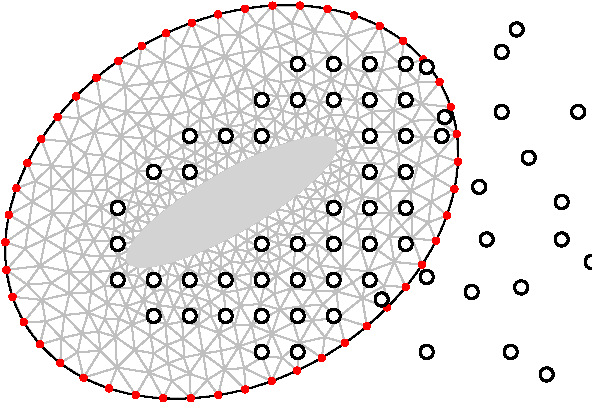
\includegraphics[width=0.5\linewidth]{./figures/hybrid/interpolation/ellipse/eulerianDirichletBC-crop.pdf}
	\caption{Dirichlet boundary conditions at boundary of Eulerian domain $\mathbf{u} \in \partial \Omega_E$. We evaluate the induced velocities from the Lagrangian solution at the nodes of the boundary  [{\color{plotRed}{$\bullet$}}, red dot].}
	\label{fig:eulerianDirichletBC}
	\end{figure}	


\subsection{Multi-step evolution}
\label{subsec:mse}
% Evolution, neglect the pressure b.c, and evolve the problem
% sub

When coupling the Eulerian solver with the Lagrangian solver, we will see that the Eulerian time step size $\Delta t_E \leqslant \Delta t_L$. This is also the main benefit of the domain decomposition such that the wake region can be evolved with much larger step size. So we will have to perform $k_E$ Eulerian sub-steps to reach the Lagrangian step $t_{n+1}$,
\begin{equation}
t_{k} = t_n + k\Delta t_E,
\end{equation}
where $k = 0,...,k_E$ and $k_E$ is given as
\begin{equation}
k_E = \frac{t_{n+1}-t_{n}}{\Delta t_E} = \frac{\Delta t_L}{\Delta t_E}.
\label{eq:timeStepDependency}
\end{equation}
When $k=0$, we have $t_k = t_n$ and for $k=k_E$, we have $t_k = t_{n+1}$. We have a criterion that $\Delta t_L$ must be multiple of $\Delta t_E$ for an integer $k_E$. Figure \ref{fig:multiStep} depicts the multi-stepping of the Eulerian solution from $t_n$ to $t_{n+1}$ to match the Lagrangian time. As the Eulerian solver requires boundary condition at each sub-step, we have to perform a interpolation of the boundary conditions for each sub-step $t_k$. We can perform a linear interpolation of the boundary condition for determines the boundary conditions at each sub-step,
\begin{equation}
\mathbf{u}(t_k) = \mathbf{u}(t_n) + k \Delta \mathbf{u},
\end{equation}
where $\Delta \mathbf{u}$ is given as
\begin{equation}
\Delta \mathbf{u} = \frac{\mathbf{u}(t_{n+1})-\mathbf{u}(t_n)}{k_E},
\end{equation}
and is the gradient in velocity between each sub-step. We can summarized the feature of the evolution of the Eulerian solution as follows:
\begin{itemize}
\item The Eulerian solver uses a $1^{st}$ order Forward Euler time-marching scheme to evolution the solution from $t_n$ to $t_k$.
\item The solution is evolved $k_E$ steps to reach $t_{n+1}$.
\item We use velocity-pressure $\mathbf{u}-p$ formulation for the solution in the Eulerian solver.
\item At the end of the time-step $t_{n+1}$, the Eulerian solver will have a higher resolved solution of the wall-region in comparison to the Lagrangian solver.
\end{itemize}

The modified correction strategy is iterated until we reach the desired time $t$.

	\begin{figure}[!t]
	\centering
	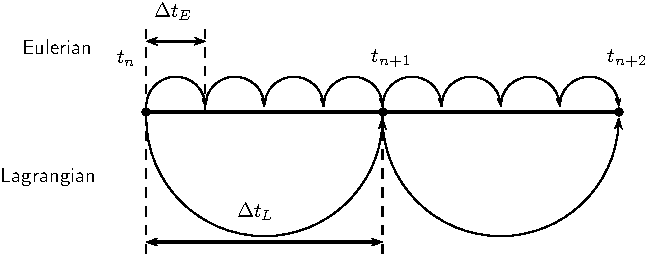
\includegraphics[width=0.7\linewidth]{./figures/eulerian/multiStep-crop.pdf}
	\caption{Eulerian multi-stepping to match the Lagrangian $\Delta t_L$. The figures shows $\Delta t_L = 4 \Delta t_E$ and required $k_E = 4$ iterations to time march from $t_n$ to $t_{n+1}$.}
	\label{fig:multiStep}
	\end{figure}


Chapter \ref{ch:eulerian} gives a detailed analysis on procedures of the Eulerian solver.
